\documentclass[a4paper,12pt]{article}
\usepackage{listing}
\usepackage{graphicx}
\begin{document}    
\title{Distance Vector Routing}
\author{Santhisenan A}
\date{\today}
\maketitle

\section{Distance Vector Routing}
A distance-vector routing protocol in data networks determines the best route for 
data packets based on distance. Distance-vector routing protocols measure the distance by
the number of routers a packet has to pass, one router counts as one hop. Some 
distance-vector protocols also take into account network latency and other factors
that influence traffic on a given route. To determine the best route across a network
routers on which a distance-vector protocol is implemented exchange information with one another,
usually routing tables plus hop counts for destination networks and possibly other traffic information.
Distance-vector routing protocols also require that a router informs its neighbours of network topology 
changes periodically.

Distance-vector routing protocols use the Bellman–Ford algorithm and 
Ford–Fulkerson algorithm to calculate the best route. Another way of calculating 
the best route across a network is based on link cost, and is implemented through l
ink-state routing protocols.

The term distance vector refers to the fact that the protocol manipulates 
vectors (arrays) of distances to other nodes in the network. The distance vector
 algorithm was the original ARPANET routing algorithm and was implemented more widely 
 in local area networks with the Routing Information Protocol (RIP).
\subsection{Code}

\begin{verbatim}
    #include<stdio.h>
    #include<iostream>
    
    using namespace std;                                            
    
    struct node
    {
        unsigned dist[6];
        unsigned from[6];
    } DVR[10];
    
    int main()
    {
    int costmat[6][6];
    int nodes, i, j, k;
    int graph1[3][3]={{0 ,1, 2 },{1, 0, 4 },{ 2 ,4 ,0 }};
    
    for(i = 0; i < 3; i++)
     {
        for(j = 0; j < 3; j++)
        {
            graph1[i][j];
            costmat[i][i] = 0;
            DVR[i].dist[j] = graph1[i][j]; 
            DVR[i].from[j] = j;
        }
    }
            for(i = 0; i < 3; i++) 
            for(j = i+1; j < 3; j++)
            for(k = 0; k < 3; k++)
                if(DVR[i].dist[j] > graph1[i][k] + DVR[k].dist[j])
                {   
                    DVR[i].dist[j] = DVR[i].dist[k] + DVR[k].dist[j];
                    DVR[j].dist[i] = DVR[i].dist[j];
                    DVR[i].from[j] = k;
                    DVR[j].from[i] = k;
                }
        for(i = 0; i < 3; i++)
        {
            cout<<"\n\n For router: "<<i+1;
            for(j = 0; j < 3; j++)
                cout<<"\t\n node "<<j+1<<" via "<<DVR[i].from[j]+1<<" Distance "<<DVR[i].dist[j];
        }
    cout<<" \n\n ";
    return 0;
    }
\end{verbatim}

\section{Output}
\begin{figure}
    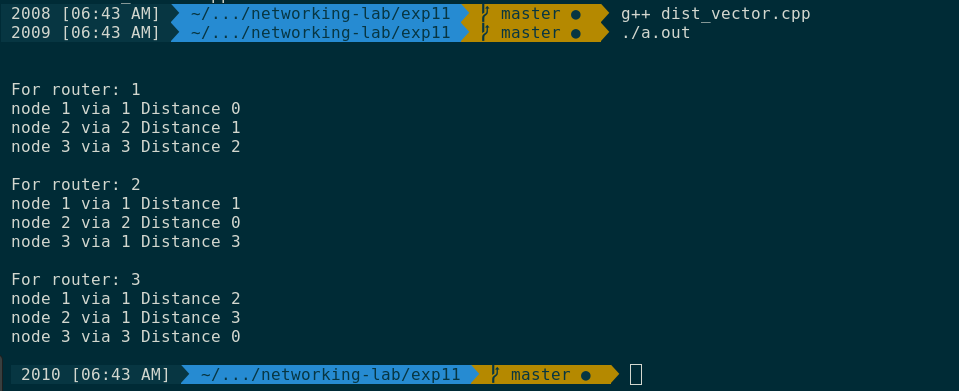
\includegraphics[width=\linewidth]{dist-vector.png}
    \caption{Distance Vector Routing}
    \end{figure}

\end{document}

